% Copyright 2004 by Till Tantau <tantau@users.sourceforge.net>.
%
% In principle, this file can be redistributed and/or modified under
% the terms of the GNU Public License, version 2.
%
% However, this file is supposed to be a template to be modified
% for your own needs. For this reason, if you use this file as a
% template and not specifically distribute it as part of a another
% package/program, I grant the extra permission to freely copy and
% modify this file as you see fit and even to delete this copyright
% notice. 

\documentclass{beamer}

\usepackage{graphicx}
\usepackage[frenchb]{babel}
\usepackage[T1]{fontenc}
\usepackage[utf8]{inputenc}
\usepackage{hyperref}
\usepackage{verbatim}
\usepackage{upquote}
\usepackage{listings}

% There are many different themes available for Beamer. A comprehensive
% list with examples is given here:
% http://deic.uab.es/~iblanes/beamer_gallery/index_by_theme.html
% You can uncomment the themes below if you would like to use a different
% one:
%\usetheme{AnnArbor}
%\usetheme{Antibes} %comme pour Georgi
%\usetheme{Bergen}
%\usetheme{Berkeley}
%\usetheme{Berlin}
%\usetheme{Boadilla}
%\usetheme{boxes}
%\usetheme{CambridgeUS}
%\usetheme{Copenhagen}
%\usetheme{Darmstadt}
%\usetheme{default}
\usetheme{Frankfurt}
%\usetheme{Goettingen}
%\usetheme{Hannover}
%\usetheme{Ilmenau}
%\usetheme{JuanLesPins}
%\usetheme{Luebeck}
%\usetheme{Madrid}
%\usetheme{Malmoe}
%\usetheme{Marburg}
%\usetheme{Montpellier}
%\usetheme{PaloAlto}
%\usetheme{Pittsburgh}
%\usetheme{Rochester}
%\usetheme{Singapore}
%\usetheme{Szeged}
%\usetheme{Warsaw}

\title{Les tests de logiciel}

% A subtitle is optional and this may be deleted
\subtitle{Tests Unitaires : Xunit}

\author{Ibrahima TOUNKARA \and Jonathan TWAMBA SAIBA}
% - Give the names in the same order as the appear in the paper.
% - Use the \inst{?} command only if the authors have different
%   affiliation.

\institute{Université de Montpellier} % (optional, but mostly needed)

% - Use the \inst command only if there are several affiliations.
% - Keep it simple, no one is interested in your street address.

\date{20 Février 2017}
% - Either use conference name or its abbreviation.
% - Not really informative to the audience, more for people (including
%   yourself) who are reading the slides online

\subject{Les tests de logiciel}
% This is only inserted into the PDF information catalog. Can be left
% out. 

% If you have a file called "university-logo-filename.xxx", where xxx
% is a graphic format that can be processed by latex or pdflatex,
% resp., then you can add a logo as follows:

\pgfdeclareimage[height=1cm]{university-logo}{un.png}
\logo{\pgfuseimage{university-logo}}

% Delete this, if you do not want the table of contents to pop up at
% the beginning of each subsection:
\AtBeginSubsection[]
{
  \begin{frame}<beamer>{Table des Matières}
    \tableofcontents[currentsection,currentsubsection]
  \end{frame}
}

% Let's get started
\begin{document}

\begin{frame}
  \titlepage
\end{frame}

\begin{frame}{Tables des Matières}
  \tableofcontents
  % You might wish to add the option [pausesections]
\end{frame}

% Section and subsections will appear in the presentation overview
% and table of contents.
\section{Test logiciel}

\subsection{Introduction}

\begin{frame}[allowframebreaks]{Introduction}
  \begin{itemize}
    
  \item {\bfseries Qu’est-ce qu’un logiciel?}
    \begin{itemize}
    \item {des besoins, exprimés par un client;}
    \item{une gestion de projet :}
      \begin{itemize}
      \item {cycle de vie (classique, agile, ...) avec ses délivrables}
      \item{les outils et l’environnement de développement}
      \end{itemize}
    \item{une spécification (fonctionalités, contraintes, facteur de qualité, interface);}
    \item{une conception : globale, architecturale, détaillée. Les composants et leurs échanges sont définis;}
    \item{un code source;}
    \item{un exécutable (un prodit);}
    \item{... {\color {blue} et des tests !}}
    \end{itemize} 
  
  \item {\bfseries Qu’est-ce que tester un logiciel? \\}
    \begin{itemize}
      {\bfseries Définition possible : }“Processus d’analyse d’un programme avec l’intention de détecter des anomalies dans le but de le valider” \\
      {\bfseries Tester un logiciel : }C’est valider sa conformité, par rapport à des exigences c’est-à-dire par rapport à l’ensemble de la spécification, et de la conception du logiciel.
    \end{itemize}

  \end{itemize}
\end{frame}

\subsection{Types}

% You can reveal the parts of a slide one at a time
% with the \pause command:
\begin{frame}{Types}
  \begin{itemize}
    
  \item{Test fonctionel\pause}
  \item{Test non fonctionnel\pause}
  \item{Test structurel}
    
  \end{itemize}
\end{frame}

\subsection{Niveaux}

% You can reveal the parts of a slide one at a time
% with the \pause command:
\begin{frame}{Niveaux}
  \begin{itemize}
    
  \item{Tests unitaires ou tests de composants \pause}
  \item{Test d'intégration\pause}
  \item{Test fonctionnel\pause}
  \item{Test Système\pause}
  \item{Test d'acceptation\pause}
  \item{Les Beta-Tests\pause}
  \item{Test de regression}
    
  \end{itemize}
\end{frame}
\begin{frame}{Niveaux}
  \begin{center}
  \let\oldtabular=\tabular 
\def\tabular{\small\oldtabular}
  \begin{tabular}{|p{1.5cm}|p{3cm}|p{1.5cm}|p{2cm}|}
  \hline
  \bfseries Test & \bfseries Portée & \bfseries Catégorie & \bfseries Exécutant \\
  \hline 
  Unitaires & Petites portions du code source & Boite noire & Développeur machine\\
  \hline 
  Intégration & Classes/composants & Boite blanche/ noire & Développeur \\
  \hline 
  Fonctionnel & Produit & Boite noire & Testeur \\
  \hline 
  Système & Produit/simulation de situation & Boite noire & Testeur  \\
  \hline 
  Acceptation & Produit/utilisation réelle & Boite noire & Client \\
  \hline 
  Béta & Produit/ Utilisation réelle & Boite noire & client\\
  \hline 
  Régression & N'importe lequel & Boite blanche/ noire & Peu importe\\
  \hline
\end{tabular}
\end{center}
\end{frame}

\begin{frame}{Niveaux}
    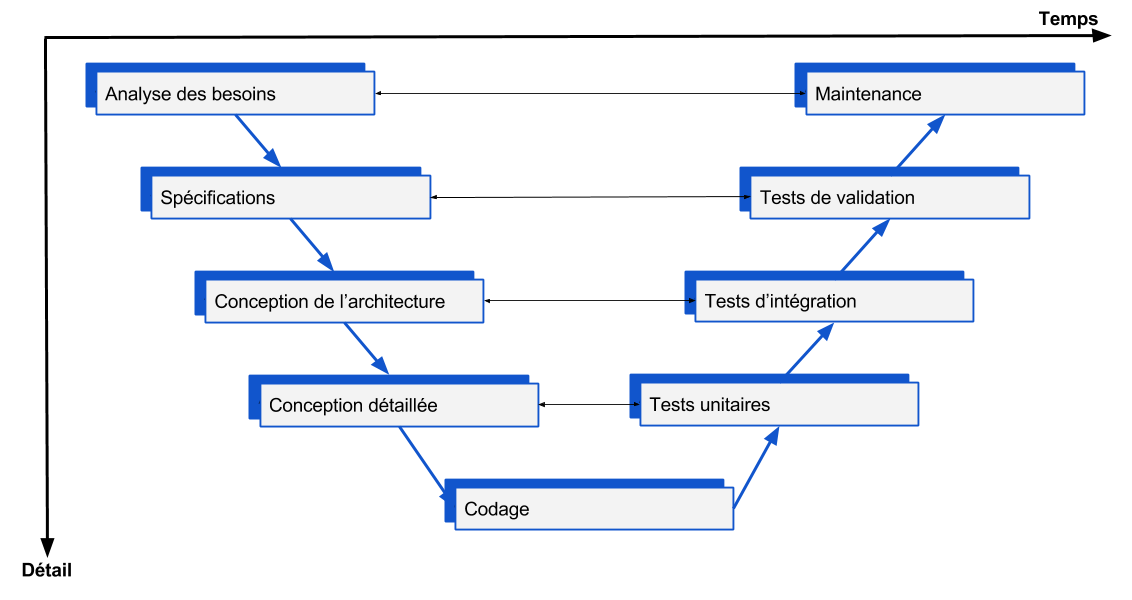
\includegraphics[width=10cm, height=8cm]{un2.png}
\end{frame}

\subsection{Objectifs}

\begin{frame}{Objectifs}

  \begin{itemize}
    
  \item{Son objectif principal est d'identifier un nombre maximum de comportements problématiques du logiciel afin d'en augmenter la qualité.\pause}
  \item{Le test peut aussi avoir pour objectif d'apporter des informations quant à cette qualité afin de permettre la prise de décisions.\pause}
  \item{Les tests de vérification ou de validation visent ainsi à vérifier que ce système réagit de la façon prévue par ses développeurs ou est conforme aux besoins du client.
}
 \end{itemize}   
\end{frame}

\begin{frame}{Objectifs}

  \begin{itemize}

  \item{Un test ressemble à une expérience scientifique. Il examine une hypothèse exprimée en fonction de trois éléments : les données en entrée, l'objet à tester et les observations attendues. \pause}

 
  \item{Eliminer les défauts qui conduisent à des défaillances avant que le logiciel entre en service}
  \item{S'assurer que le logiciel satisfait un certain nombre légal ou contractuel nécessaire pour une certification du logiciel par exemple.}
    
  \end{itemize}   
\end{frame}

\subsection{Quelques principes de Test}

\begin{frame}{Quelques principes de Test}
  \begin{itemize}
  
  \item{{\bfseries Montrer la présence de défauts}
 \\Il est important de savoir que les tests ne peuvent pas prouver qu'il n'y a pas d'erreurs mais plutôt de montrer la présence de défauts pour pouvoir les corriger. Il est important de faire des tests pertinents avant de conclure qu'il n'a pas de défauts.\pause}
  \item{{\bfseries Tester raisonnablement}
  \\Tester un logiciel ne signifie pas tester tous les états de celui-ci. Il est donc important de se concentrer sur l'essentiel; car pour certain programme c'est théoriquement impossible vu le temps que ça prendrait.}
  \end{itemize} 
\end{frame}
  \begin{frame}{Quelques principes de Test}
  \begin{itemize}
  \item{{\bfseries Tester tôt}
\\Les tests doivent commencer plus tôt pour pouvoir retrouver les erreurs plus vites et ainsi les corriger car les difficultés de correction augmentent avec la progression.\pause} 
  \item{{\bfseries Regrouper les défauts}
 \\ Il faut répartir uniformémént les tests pour ne pas oublier certaines parties du logiciel. Si l'on divise le logiciel en des parties, on remarquera que 80\% des erreurs de celui-ci sont sont concentrées dans 20\% des parties, c'est la règle du 80/20. Il faudra ainsi agir en conséquence sur les 80\%. }
 \end{itemize} 
\end{frame}
 \begin{frame}{Quelques principes de Test}
  \begin{itemize}
  \item{{\bfseries Tester des parties bien définies du Logiciel}
 \\Après avoir testé longtemps, le nombre d'erreurs va en décroisssant. Il est important de choisir donc la méthode de test appropriée pour chaque partie de logiciels et constamment renouveler les tests en changeant de point de vue. \pause}

  \item{{\bfseries Tester selon le contexte}
  \\Certains logiciels peuvent être utilisés dans des contexte différents.Par exemple, un système de gestion de bases de données peut être utilisé pour mémoriser des transactions bancaires. En fonction de l'utilisation du composant, les objectifs et les types de test ne seront pas forcément les mêmes.Les paramètres temps et environnement peuvent beaucoup jouer. }
  \end{itemize} 
  
\end{frame}
\begin{frame}{Quelques principes de Test}
  \begin{itemize}
  \item{{\bfseries Respectez les normes}
 \\Il faut le rappeler, les tests sont là pour découvrir des défauts par rapport à ce que l'on attend du logiciel. Mais il ne suffit pas  de répérer et de corriger toutes les erreurs du logiciel, il faut le rendre utilisable.L'absence de défauts sous un angle particulier ne garantira pas une bonne qualité sous un autre. Les différents attendus du logiciels doivent correspondre à la norme ISO 9126 dont les critères principaux sont: Fonctionnality, Usability, Reliability, Portability, Efficiency, Maintainability.}
    
\end{itemize} 
\end{frame}

% You can reveal the parts of a slide one at a time
% with the \pause command:

\section{Tests Unitaires: XUNIT}

\subsection{Introduction}

\begin{frame}{Introduction}
  \begin{itemize}
    
  \item{Les tests unitaires sont des tests en boîte blanche}
  \item{Les tests unitaires sont composés d'un ensemble de classes appelées "{\color{blue}classes de test}"}
  \item{Ces classes valident que des portions de code répondent à un certain besoin}
  \item{Les tests unitaires sont importants car ils permettent de détecter le maximum de défaillance avant les tests en boîte noire et qu'ils peuvent s'exécuter d'une manière automatique}
    
  \end{itemize}   
\end{frame}

\subsection{Objectifs}

\begin{frame}{Objectifs}
  \begin{itemize}
    
  \item{Les tests unitaires ont deux objectifs : "{\color{blue} couveture de code}" et "{\color{blue}couverture de données}"}
  \item{La couverture du code stipule de tester chaque ligne de code écrite (appel de fonction, boucles, décisions, décisions multiples, ...}
  \item{La couverture des données oriente les tests vers les données (donnéess valides, données invalides, accès aux éléments en dehors de la capacité d'un tableau, peu de données, trop de données,... etc)}
    
  \end{itemize}   
\end{frame}

\subsection{Les frameworks de type xUnit}

\begin{frame}{Les frameworks de type xUnit}
Pour écrire des tests unitaires, vous avez à votre disposition des frameworks qui vont vous faciliter l'écriture des tests. Vous n'aurez plus qu'à écrire les classes de tests et c'est le framework qui se chargera de les trouver, de les lancer et de vous donner les résultats ou les erreurs qui ont été détectées. \\

  \begin{itemize}
  \item{{\bfseries En Java} : {\href{http://junit.org/junit4/}{JUnitest}} le framework de type xUnit le plus utilisé pour Java. Il est tellement utilisé qu'il est livré avec la plupart des IDE.} 
  \end{itemize}   
\end{frame}
  \begin{frame}
  \begin{itemize}
  \item{{\bfseries En C++} : Cutte, Google propose Google C++ Testing Framework, la fameuse bibliothèque Boost comprend la Boost Test Library.}
  \item{{\bfseries En Python} : la distribution de base de Python intègre unittest mais il existe aussi PyUnit.}
  \item{{\bfseries En PHP} : les développeurs PHP utilisent PHPUnit (ex: Zend Framework, Drupal V8[2]); SimpleTest (ex: Drupal V7[3]) qui possède une documentation en français; Atoum.}
  \item{{\bfseries En Ruby} : Ruby intègre Test::Unit} 
  \end{itemize}   
\end{frame}
  \begin{frame}
  \begin{itemize}
  \item{{\bfseries En D} : le langage intègre nativement le mot-clé unittest.}
  \item{{\bfseries En Groovy} : voir Unit Testing}
  \item{{\bfseries En JavaScript} : le framework jQuery utilise qunit, Jarvis, jfUnit, google-js-test}
  \item{{\bfseries Dans d'autres langages} : il existe des frameworks équivalents dans la plupart des langages : vous pouvez les découvrir dans l'article « List of unit testing frameworks » sur Wikipedia anglophone.}

  \end{itemize}
\end{frame}
    
\subsection{JUnit}

\begin{frame}{JUnit}
    \begin{itemize}
        \item{{\bfseries Écrire un test} : Avec JUnit, on va créer une nouvelle classe pour chaque classe testée. On crée autant de méthodes que de tests indépendants : imaginez que les tests peuvent être passés dans n'importe quel ordre (i.e. les méthodes peuvent être appelées dans un ordre différent de celui dans lequel elles apparaissent dans le code source). Il n'y a pas de limite au nombre de tests que vous pouvez écrire. Néanmoins, on essaye généralement d'écrire au moins un test par méthode de la classe testée. Pour désigner une méthode comme un test, il suffit de poser l'annotation {\color{blue}@Test}.}
        \end{itemize}   
\end{frame}
\begin{frame}{JUnit}
   \lstinputlisting[language=Java]{bcb.java}
   \end{frame}
  \begin{frame}{JUnit}
   \begin{itemize}
       \item{{\bfseries Les assertions}
    \\Via {\color{blue}import static org.junit.Assert.* };, vous devez faire appel
    dans les tests aux méthodes statiques assertTrue, assertFalse,
    assertEquals, assertNull, fail, etc. en fournissant un message.
    Votre environnement de développement devrait vous permettre
    de découvrir leurs signatures grâce à l’auto-complétion. À
    défaut, vous pouvez toutes les retrouver dans la
    documentation de l’API JUnit.   
Attention à ne pas confondre les assertions JUnit avec
«assert». Ce dernier est un élément de base du langage
Java.}%Par défaut, les assertions Java sont ignorées par la
%JVM à moins de préciser -ea au lancement de la JVM}
    \end{itemize}
   \end{frame}
       
    \begin{frame}{JUnit}   
    \begin{itemize}
    \item{\bfseries Lancer les tests} :\\
       Pour lancer les tests, vous avez plusieurs possibilités selon vos préférences:
       \begin{itemize}
      
        \item{La plus courante : lancer les tests depuis votre IDE}
        \item{Utiliser l'outil graphique}
        \item{Lancer les tests en ligne de commande}
        \item{Utiliser un système de construction logiciel (comme Ant ou Maven pour Java)}
        \end{itemize}
        \end{itemize}
    \end{frame}
        
         \begin{frame}{JUnit}   
         \begin{itemize}
        \item{{\bfseries Factoriser les éléments communs entre tests} :\\
        On peut déjà chercher à factoriser les éléments communs à tous les tests d'une seule classe. Un test commence toujours par l'initialisation de quelques instances de formes différentes pour pouvoir tester les différents cas. C'est souvent un élément redondant des tests d'une classe, aussi, on peut factoriser tout le code d'initialisation commun à tous les tests dans une méthode spéciale, qui sera appelée avant chaque test pour préparer les données.
        Si on considère l'exemple ci-dessus, cela donne :}
        
         \end{itemize}
         \end{frame}
            
         \begin{frame}[allowframebreaks]
         \begin{small}
         \lstset{small}
        \lstinputlisting[language=Java]{bcc.java}
        
        \end{small}
        \end{frame}
       
        \begin{frame}{JUnit}   
         \begin{itemize}
        \item{{\bfseries Écrire de bon tests } : 
        Idéalement, les tests unitaires testent une classe et une seule et sont indépendants les uns des autres. En effet, si une classe A est mal codée et qu'elle échoue au test unitaire de A, alors B qui dépend de A (parce qu'elle manipule des instances de A ou hérite de A) va probablement échouer à son test alors qu'elle est bien codée.\\
        Selon les langages, on a souvent des conventions pour nommer les classes de tests. En Java, on choisit souvent d'appeler {\color{blue}MaClassTest} le test de la classe MaClass. Les tests peuvent être commentés si le déroulement d'un test est complexe.\\
        Évidemment, un bon test assure la qualité de l'intégralité d'une classe, et pas seulement d'une partie de celle-ci.}
    
   \end{itemize}
  
\end{frame}

% Placing a * after \section means it will not show in the
% outline or table of contents.

\section{Conclusion}

\subsection{Conclusion}

\begin{frame}{Conclusion}
Différentes stratégies de tests peuvent être mise en oeuvre pour tester un logiciel.
Comme nous l'avons vu, les tests doivent être un guide lors des différentes phases du projet et ceci quelque soit le cycle de développement retenu pour rendre le logiciel plus simple à concevoir et à exécuter durant les phases de réalisation, de déploiement ou de maintenace du logiciel.


\end{frame}
\begin{frame}{Conclusion}
\begin{center}
Merci de votre attention!
\end{center}
\end{frame}

% Placing a * after \section means it will not show in the
% outline or table of contents.
% All of the following is optional and typically not needed.

\appendix

\section<presentation>*{\appendixname
}
\subsection<presentation>*{Bibliographie}

\begin{frame}[allowframebreaks]
  \frametitle<presentation>{Bibliographie}
    
  \begin{thebibliography}{10}
    \beamertemplatebookbibitems
  % Start with overview books.

  \bibitem{Author2014}
    Jean-François Pradat-Peyre.
    \newblock {\em Pratique des tests logiciels.}
    \newblock DUNOD, 2014.
 
    
  \bibitem{Author2010}
    John Dooley.
    \newblock {\em Software Development and Professionnel Pratice.}
    \newblock APress, 2010.
    
    \beamertemplatearticlebibitems
  % Followed by interesting articles. Keep the list short. 

  \bibitem{Someone2011}
    F.X. Fornari.
    \newblock Introduction aux tests du logiciel.
    \newblock {\em https://www.irif.fr/~eleph/Enseignement/2010-11/CoursTests.pdf, 2011.}

  \bibitem{Someone2000}
    Merlyn Albery-Speyer.
    \newblock Ten commandments of unit testing.
    \newblock {\em https://monkeyisland.pl/2008/01/31/10rules/http://www.curiousattemptbunny.com/2007/11/ten-commandments-of-unit-testing.html, 2011.}
    
  \end{thebibliography}
\end{frame}

\end{document}

